% ─────────────────────────────────────────────────────────────────────────────
\section{Background}
% ─────────────────────────────────────────────────────────────────────────────

\paragraph{Agent-Based Modelling and Multi-Agent Systems}
ABM is a powerful tool for studying complex systems by simulating the behaviours of autonomous individuals \citep{ar:Schelling1971,ar:Macal2016}. This approach allows macro-level phenomena to emerge from simple micro-level rules. A classic example is Reynolds' boids model, where agents follow basic steering rules, such as separation and alignment, to produce coherent flocking patterns \citep{inpr:Reynolds1987}. In the context of SAR, this framework provides a way to analyse how individual agent-level choices translate into collective search efficiency.

\paragraph{Belief-Desire-Intention Architecture}
The BDI architecture is a common framework for designing rational agents \citep{bk:Bratman1987,inpr:RaoGeorgeff1991}. In this model, beliefs represent the information an agent has about its environment. Desires are the long-term objectives the agent wants to achieve. Intentions are the specific plans the agent commits to executing in order to fulfil its desires based on its current beliefs. This architecture allows agents to balance goal-oriented behaviour with the flexibility to react to new information from their sensors.

\paragraph{Ant Colony Optimization and Stigmergy}
Coordination in MAS is often achieved through stigmergy, where agents communicate indirectly by modifying their shared environment \citep{bk:Bonabeau1999}. ACO is a well-known metaheuristic inspired by this principle \citep{ar:Dorigo1996,bk:Dorigo2004}. In natural ant colonies, individuals deposit pheromones on the ground to mark successful paths to food sources. Future agents are attracted to these markers, which creates a positive feedback loop that leads the group toward efficient solutions. This coordination mechanism requires no direct communication between agents and is highly effective for solving complex spatial search problems.

% ─────────────── full-width statechart figure ─────────────────────────────
\begin{figure*}[ht]
    \centering
    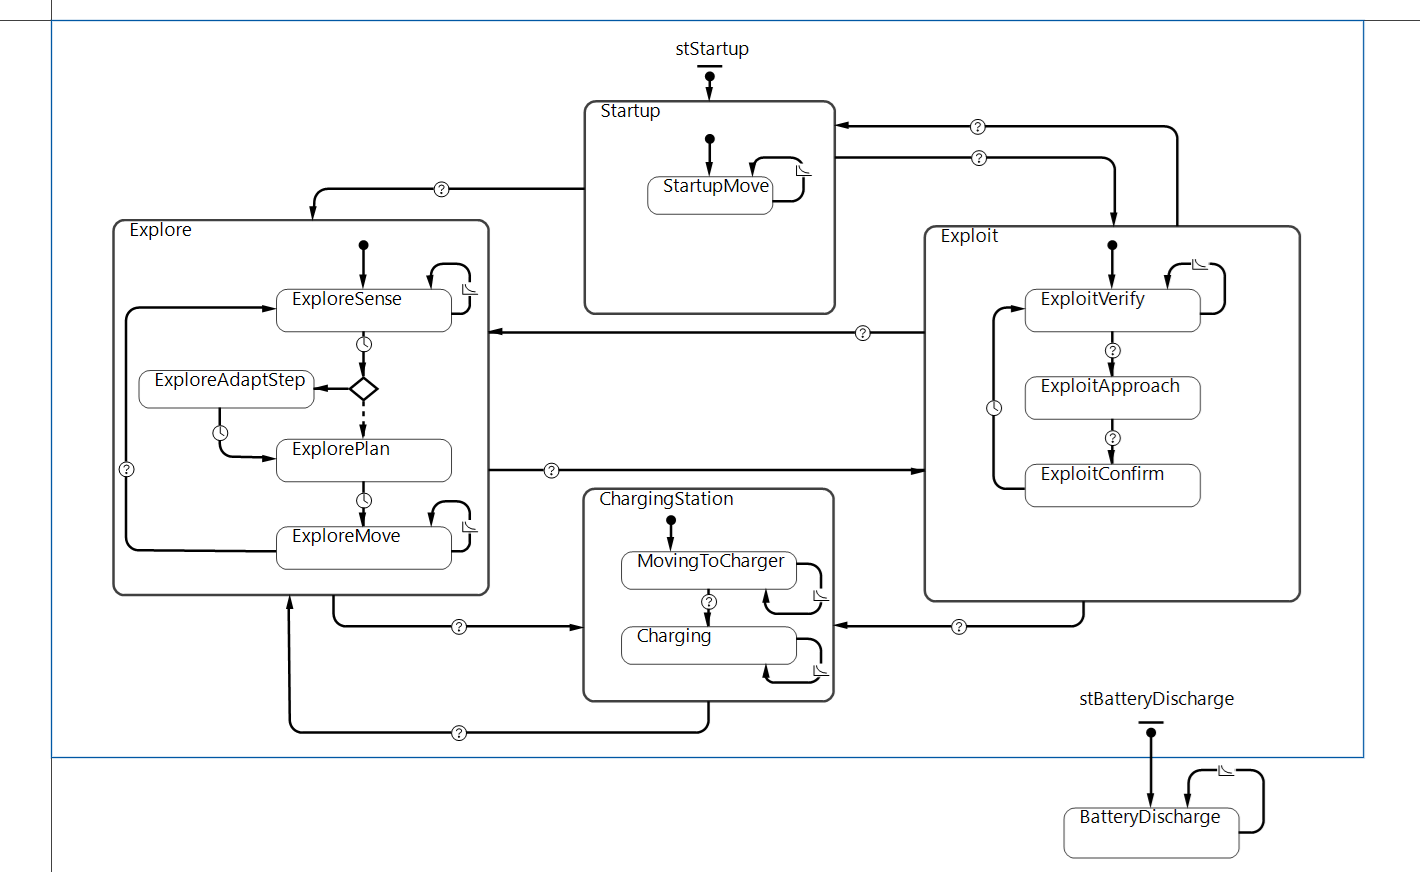
\includegraphics[width=\textwidth]{img/statechart.png}
    \caption{The BDI-inspired UAV statechart shows the primary behavioral modes. The \texttt{Startup} mode manages the movement to initial dispersal points. The \texttt{Explore} mode uses pheromone logic to search the environment. The \texttt{Exploit} mode handles victim confirmation and approach. The \texttt{ChargingStation} mode handles battery replenishment at the base. Finally, the \texttt{BatteryDischarge} state runs in parallel to simulate continuous energy consumption.}
    \label{fig:statechart}
\end{figure*}
